\section{Independence}

Suppose that we flip two fair coins simultaneously on opposite sides
of a room.  Intuitively, the way one coin lands does not affect the
way the other coin lands.  The mathematical concept that captures
this intuition is called \term{independence}:
\begin{definition*}
Events $A$ and $B$ are independent if and only if:
\[
\pr{A \intersect B} = \pr{A} \cdot \pr{B}
\]
\end{definition*}
Generally, independence is something you \textit{assume} in modeling a
phenomenon--- or wish you could realistically assume.  Many useful
probability formulas only hold if certain events are independent, so a
dash of independence can greatly simplify the analysis of a system.

\subsection{Examples}

Let's return to the experiment of flipping two fair coins.  Let $A$ be
the event that the first coin comes up heads, and let $B$ be the event
that the second coin is heads.  If we assume that $A$ and $B$ are
independent, then the probability that both coins come up heads is:
%
\begin{align*}
\pr{A \intersect B} & = \pr{A} \cdot \pr{B} \\
              & = \frac{1}{2} \cdot \frac{1}{2} \\
              & = \frac{1}{4}
\end{align*}

On the other hand, let $C$ be the event that tomorrow is cloudy and
$R$ be the event that tomorrow is rainy.  Perhaps $\pr{C} = 1/5$ and
$\pr{R} = 1/10$ around here.  If these events were independent, then
we could conclude that the probability of a rainy, cloudy day was
quite small:
%
\begin{align*}
\pr{R \intersect C} & = \pr{R} \cdot \pr{C} \\
              & = \frac{1}{5} \cdot \frac{1}{10} \\
              & = \frac{1}{50}
\end{align*}
%
Unfortunately, these events are definitely not independent; in
particular, every rainy day is cloudy.  Thus, the probability of a
rainy, cloudy day is actually $1/10$.

\subsection{Working with Independence}

There is another way to think about independence that you may find more
intuitive.  According to the definition, events $A$ and $B$ are
independent if and only if $\pr{A \intersect B} = \pr{A} \cdot \pr{B}$.  This
equation holds even if $\pr{B} = 0$, but assuming it is not, we can divide
both sides by $\pr{B}$ and use the definition of conditional probability
to obtain an alternative formulation of independence:
\begin{proposition*}
If $\pr{B} \neq 0$, then
events $A$ and $B$  are independent if and only if
\begin{equation}\label{LN12:ABA}
\prcond{A}{B} = \pr{A}.
\end{equation}
\end{proposition*}

Equation~\eqref{LN12:ABA} says that events $A$ and $B$ are independent if the
probability of $A$ is unaffected by the fact that $B$ happens.  In these
terms, the two coin tosses of the previous section were independent,
because the probability that one coin comes up heads is unaffected by the
fact that the other came up heads.  Turning to our other example, the
probability of clouds in the sky is strongly affected by the fact that it
is raining.  So, as we noted before, these events are not independent.

\textbf{Warning:} Students sometimes get the idea that disjoint events are
independent.  The \emph{opposite} is true: if $A \intersect B =
\emptyset$, then knowing that $A$ happens means you know that $B$ does not
happen.  So disjoint events are \emph{never} independent ---unless one of
them has probability zero.
\iffalse

\subsection{Some Intuition}

Suppose that $A$ and $B$ are disjoint events, as shown in the figure
below.
%
\begin{center}
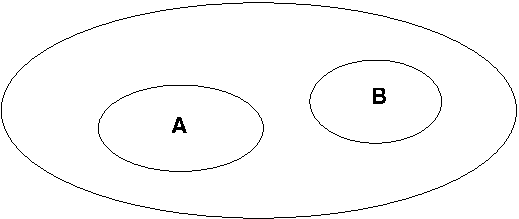
\includegraphics{figures/disjoint-events}
\end{center}
%
Are these events independent?  Let's check.  On one hand, we know
%
\[
\pr{A \intersect B} = 0
\]
%
because $A \intersect B$ contains no outcomes.  On the other hand, we have
%
\[
\pr{A} \cdot \pr{B} > 0
\]
%
except in degenerate cases where $A$ or $B$ has zero probability.
Thus, \textit{disjointness and independence are very different ideas}.

Here's a better mental picture of what independent events look like.
%
\begin{center}
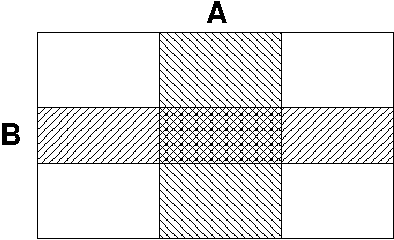
\includegraphics{figures/independent-events}
\end{center}
%
The sample space is the whole rectangle.  Event $A$ is a vertical
stripe, and event $B$ is a horizontal stripe.  Assume that the
probability of each event is proportional to its area in the diagram.
Now if $A$ covers an $\alpha$-fraction of the sample space, and $B$
covers a $\beta$-fraction, then the area of the intersection region is
$\alpha \cdot \beta$.  In terms of probability:
%
\[
\pr{A \intersect B} = \pr{A} \cdot \pr{B}
\]
\fi

\subsection{Mutual Independence}

We have defined what it means for two events to be independent.  But
how can we talk about independence when there are more than two
events?  For example, how can we say that the orientations of $n$
coins are all independent of one another?

Events $E_1, \ldots, E_n$ are \term{mutually independent} if and only
if \textit{for every subset} of the events, the probability of the
intersection is the product of the probabilities.  In other words, all
of the following equations must hold:
%
\begin{align*}
\pr{E_i \intersect E_j}
    & = \pr{E_i} \cdot \pr{E_j}
    & \text{for all distinct $i$, $j$} \\
\pr{E_i \intersect E_j \intersect E_k}
    & = \pr{E_i} \cdot \pr{E_j} \cdot \pr{E_k}
     & \text{for all distinct $i$, $j$, $k$} \\
\pr{E_i \intersect E_j \intersect E_k \intersect E_l}
    & = \pr{E_i} \cdot \pr{E_j} \cdot \pr{E_k} \cdot \pr{E_l}
    & \text{for all distinct $i$, $j$, $k$, $l$} \\
    & \ldots \\
\pr{E_1 \intersect \cdots \intersect E_n} & = \pr{E_1} \cdots \pr{E_n}
\end{align*}
%
As an example, if we toss 100 fair coins and let $E_i$ be the event
that the $i$th coin lands heads, then we might reasonably assume that
$E_1, \ldots, E_{100}$ are mutually independent.

\iffalse

\subsection{DNA Testing}

This is testimony from the O. J. Simpson murder trial on May 15, 1995:

\textbox{
\begin{description}

\item[MR. CLARKE:] When you make these estimations of frequency--- and
I believe you touched a little bit on a concept called independence?

\item[DR. COTTON:] Yes, I did.

\item[MR. CLARKE:] And what is that again?

\item[DR. COTTON:] It means whether or not you inherit one allele that
you have is not--- does not affect the second allele that you might
get.  That is, if you inherit a band at 5,000 base pairs, that doesn't
mean you'll automatically or with some probability inherit one at
6,000.  What you inherit from one parent is what you inherit from the
other.  \emph{(Got that? -- EAL)}

\item[MR. CLARKE:] Why is that important?

\item[DR. COTTON:] Mathematically that's important because if that
were not the case, it would be improper to multiply the frequencies
between the different genetic locations.

\item[MR. CLARKE:] How do you--- well, first of all, are these markers
independent that you've described in your testing in this case?

\end{description}
}

The jury was told that genetic markers in blood found at the crime
scene matched Simpson's.  Furthermore, the probability that the
markers would be found in a randomly-selected person was at most 1 in
170 million.  This astronomical figure was derived from statistics such
as:
%
\begin{itemize}
\item 1 person in 100 has marker $A$.
\item 1 person in 50 marker $B$.
\item 1 person in 40 has marker $C$.
\item 1 person in 5 has marker $D$.
\item 1 person in 170 has marker $E$.
\end{itemize}
%
Then these numbers were multiplied to give the probability that a
randomly-selected person would have all five markers:
%
\begin{align*}
\pr{A \intersect B \intersect C \intersect D \intersect E}
    & = \pr{A} \cdot \pr{B} \cdot \pr{C} \cdot \pr{D} \cdot \pr{E} \\
    & = \frac{1}{100} \cdot \frac{1}{50} \cdot \frac{1}{40}
                      \cdot \frac{1}{5} \cdot \frac{1}{170} \\
    & = \frac{1}{170,000,000}
\end{align*}
%
The defense pointed out that this assumes that the markers appear
mutually independently.  Furthermore, all the statistics were based on
just a few hundred blood samples.  The jury was widely mocked for
failing to ``understand'' the DNA evidence.  If you were a juror,
would \textit{you} accept the 1 in 170 million calculation?
\fi

\subsection{Pairwise Independence}

The definition of mutual independence seems awfully complicated---
there are so many conditions!  Here's an example that illustrates the
subtlety of independence when more than two events are involved and
the need for all those conditions.  Suppose that we flip three fair,
mutually-independent coins.  Define the following events:
%
\begin{itemize}
\item $A_1$ is the event that coin 1 matches coin 2.
\item $A_2$ is the event that coin 2 matches coin 3.
\item $A_3$ is the event that coin 3 matches coin 1.
\end{itemize}
%
Are $A_1$, $A_2$, $A_3$ mutually independent?

The sample space for this experiment is:
%
\[
\set{HHH,\ HHT,\ HTH,\ HTT,\ THH,\ THT,\ TTH,\ TTT}
\]
%
Every outcome has probability $(1/2)^3 = 1/8$ by our assumption that
the coins are mutually independent.

To see if events $A_1$, $A_2$, and $A_3$ are mutually independent, we
must check a sequence of equalities.  It will be helpful first to
compute the probability of each event $A_i$:
%
\begin{align*}
\pr{A_1} & = \pr{HHH} + \pr{HHT} + \pr{TTH} + \pr{TTT} \\
         & = \frac{1}{8} + \frac{1}{8} + \frac{1}{8} + \frac{1}{8}\\
         & = \frac{1}{2}
\end{align*}
%
By symmetry, $\pr{A_2} = \pr{A_3} = 1/2$ as well.  Now we can begin
checking all the equalities required for mutual independence.
%
\begin{align*}
\pr{A_1 \intersect A_2}
	& = \pr{HHH} + \pr{TTT} \\
        & = \frac{1}{8} + \frac{1}{8} \\
        & = \frac{1}{4} \\
        & = \frac{1}{2} \cdot \frac{1}{2}\\
        & = \pr{A_1} \pr{A_2}
\end{align*}
%
By symmetry, $\pr{A_1 \intersect A_3} = \pr{A_1} \cdot \pr{A_3}$ and
$\pr{A_2 \intersect A_3} = \pr{A_2} \cdot \pr{A_3}$ must hold also.
Finally, we must check one last condition:
%
\begin{align*}
\pr{A_1 \intersect A_2 \intersect A_3}      & = \pr{HHH} + \pr{TTT} \\
                                & = \frac{1}{8} + \frac{1}{8} \\
                                & = \frac{1}{4} \\
                                & \neq \pr{A_1} \pr{A_2} \pr{A_3} = \frac{1}{8}
\end{align*}
%
The three events $A_1$, $A_2$, and $A_3$ are not mutually independent,
even though all \textit{pairs} of events are independent!

A set of events is \term{pairwise independent} if every pair is
independent.  Pairwise independence is a much weaker property than mutual
independence, but we'll see some examples in later notes when pairwise
independence is all that's needed.

\iffalse
  For example, suppose that the prosecutors in the
O. J. Simpson trial were wrong and markers $A$, $B$, $C$, $D$, and $E$
appear only \textit{pairwise} independently.  Then the probability
that a randomly-selected person has all five markers is no more than:
%
\begin{align*}
\pr{A \intersect B \intersect C \intersect D \intersect E}
    & \leq \pr{A \intersect E} \\
    & = \pr{A} \cdot \pr{E} \\
    & = \frac{1}{100} \cdot \frac{1}{170} \\
    & = \frac{1}{17,000}
\end{align*}
%
The first line uses the fact that $A \intersect B \intersect C \intersect D \intersect E$ is a
subset of $A \intersect E$.  (We picked out the $A$ and $E$ markers because
they're the rarest.)  We use pairwise independence on the second line.
Now the probability of a random match is 1 in 17,000--- a far cry from
1 in 170 million!  And this is the strongest conclusion we can reach
assuming only pairwise independence.\fi

\endinput